%\documentclass[12pt,preprint]{aastex}
\documentclass[iop]{emulateapj}
\usepackage{natbib,amsmath,graphicx,longtable,amssymb,latexsym,epsf}
\begin{document}

\title{Quasars Probing Quasars IX. Probing the Circumgalactic Flows of Quasars [v1.1]}

\author{Marie Wingyee Lau\altaffilmark{1}, J. Xavier Prochaska\altaffilmark{1}, 
Joseph F. Hennawi\altaffilmark{2}
}
\altaffiltext{1}{Department of Astronomy and Astrophysics, UCO/Lick Observatory, University of 
California, 1156 High Street, Santa Cruz, CA 95064}
\altaffiltext{2}{Max-Planck-Institut f\"ur Astronomie, K\"onigstuhl 17, D-69115 Heidelberg, 
Germany} 

\begin{abstract}
Blah
\end{abstract}


\keywords{glaxies: clusters: intracluster medium -- galaxies: formation -- galaxies: halos -- 
intergalactic medium -- quasars: absorption lines -- quasars: general}

\section{Introduction}

%\begin{itemize}
%\item Flows
%\item Mass (Kaiser, Schaye)
%\item Directionality/symmetry
%\item Break the symmetry
%\end{itemize}

%Take words from my summary of SomervilleDave15. 

The formation and evolution of stars are dictated
by the flow of gas and metals/dust.  [This transport
varies directly with the stellar stage
and a lesser extent stellar mass.]
The accretion onto a protostellar  core eventually
initiates nuclear fusion.  The main sequence is characterized
by gentler stellar winds, with the most massive
stars shedding a cumulative mass of XX\%.
Stellar deaths, meanwhile, are frequently accompanied by terrific
mass loss, occasionally punctuated by a highly energetic,
supernova phase.

By analogy, galaxy formation and evolution are driven by the
flows into/out of their interstellar medium.
In contrast to most stars, however, current theories
predict (even demand) that the star-forming galaxies
maintin these flows. [add]

Akin to stars, direct observations of galactic flows are
difficult to acquire.  Even detecting the gas is challenging:
the gas mass is either too small or the gas density too low
for the [detection] of line-emission (e.g. 21cm, lya,
or H$\alpha$ from Hydrogen).  Resolving the kinematics
and establish the mass-flux represent a far greater challenge.
These challenges are accentuated for distant, young galaxies
where flows are predicted to prevail \citep{keres,fumagalli}.
Therefore, with rare exceptions \citep[e.g.][]{slug,jackpot},
the community has relied on absorption-line spectroscopy
to detect and characterize the gas surrounding galaxies
\citep[e.g.][]{bergeron,steidel10,pro11,tumlinson13}.
With this experiment, researcher have had recent success
in characterizing the large-scale flows around star-forming
galaxies to reveal a net inflow \cite{rakic13} and
provide unique constraints on the mass of the underlying
potential well \cite{rakic14}.

A significant limitation of standard absorption-line
analysis, especially regarding sutyding galactic flows,
is the inherent symmetry of the experiment.
Because one generally lacks any constraint on the distance
of the gas along the sightline,
postive or negative velocities with respect to the
galaxy may be interpreted as gas flowing either towards
or away from the system.
So-called `down-the-barrel' observations break this
symmetry, and have generally provided evidence for flows
away from galaxies \citep{rupke,martin,weiner,rubin}.
However, these data are frequently at low spectral resolution
which limits one's sensitivity to inflowing gas.

In this paper, we examine the flows of gas in the environments
of massive galaxies hosting quasars.  Our approach leverages
a large dataset of quasar pairs \citep{hennawi}
to use the standard technique of absorption-line spectroscopy
with background quasars. [word]
These quasar pairs have angular
separations that correspond to less than 300\,kpc physical
separation at the f/g quasar redshift.
Our previous publications from these quasar pairs
have established that these galaxies are surrounded
by a massive, cool, and enriched circumgalactic medium
\citep{QPQ1,QPQ5,QPQ6,QPQ7}.
We have collected a sample of ntot~spectra passing within
300\,kpc from a f/g quasar with a precisely measured
redshift.  Our primary scientific interests are twofold:
(i) search for signatures of galactic-scale outflows from the
central galaxy, presumably driven by recent star-formation
and/or AGN feedback;
(ii) characterize the dynamics of galactic flows around these
massive system.  We further descrbie an aspect of this
experiment that offers a unique opportunity to study galactic
flows. [detail??]

Throughout this manuscript we adopt a $\Lambda$CDM cosmology with $\Omega_M=0.26, \Omega_\Lambda
=0.74$, and $H_0=70\,{\rm km\,s^{-1}\,Mpc^{-1}}$. All distances are proper unless otherwise 
stated. 
%When referring to comoving distances we include explicitly an $h^{-1}$ term and 
%follow modern convention of scaling to a Hubble constant of $70\,{\rm km\,s^{-1}\,Mpc^{-1}}$. All 
%equivalent width measurements are presented in the rest-frame, unless otherwise specified. 

\section{The Experiment}
\label{sec:data}

Our primary scientific interest is to measure the average velocity fields of the C$^+$, C$^{3+}$, 
and Mg$^+$ absorption associated with the CGM of the massive galaxies hosting $z\sim 2.4$ quasars. 

From our QPQ survey\footnote{http://www.qpqsurvey.org} (QPQ1), we have analyzed a subset of  
systems that pass within 300\,kpc physical from a foreground quasar with $z > 1.6$. We restrict
 the sample to foreground quasars with redshift measured from \ion{Mg}{2}\,2800, 
[\ion{O}{3}]\,5007, H$\alpha$, or H$\beta$ emission, giving a precision of 
$400\,{\rm km\,s^{-1}}$ or lower. 
[\ion{O}{3}] emission-line redshifts have the smallest dispersion of $44\,{\rm km\,s^{-1}}$ about 
the systemic redshift, and we analyze the sub-sample with [\ion{O}{3}] redshifts separately. 
The [\ion{O}{3}] line has an average blueshift of $27\,{\rm km\,s^{-1}}$ about the systemic 
redshift \citep{Boroson05}, which has been added when we compute the 
redshift of the line. Systemic redshifts measured from \ion{Mg}{2} have a precision of 
$272\,{\rm km\,s^{-1}}$, and we have taken into account the median redshift of 
$97\,{\rm km\,s^{-1}}$ of \ion{Mg}{2} from [\ion{O}{3}] \citep{Richards+02}. In QPQ8. we have 
quantified the precision of H$\alpha$ and H$\beta$ to be 
$300\,{\rm km\,s^{-1}}$ and $392\,{\rm km\,s^{-1}}$ respectively. We further supplement the 
dataset with quasar pairs selected from the igmspec 
database\footnote{https://github.com/specdb/igmspec}, which comes with the package of software for
accessing spectra of sources useful for probing the intergalactic medium \citep{Prochaska17}. 
We reach a total of 195 sightlines in the final sample. Among them, 13 have spectral resolution 
$> 5000$ from echellette or echelle observations and have been analyzed separately in QPQ8. 
Figure~\ref{fig:experiment} summarizes the experimental design. We refer the reader to previous 
QPQ publications for the redshift centroiding algorithm, and details on data reduction and 
continuum normalization (QPQ6, QPQ8). 

As in the previous QPQ papers, we make a cut on velocity difference between the redshifts of the 
two quasars in a pair of $>3000\,{\rm km\,s^{-1}}$ to avoid physically associated binary quasars. 
The cut on velocity difference is motivated by the typical redshift uncertainty of 
$\approx500\,{\rm km\,s^{-1}}$. In QPQ8, it was required that the observed wavelengths of the 
metal ion transitions fall outside the Ly$\alpha$ forest of the background quasar. In this paper, 
we make a more aggressive Ly$\alpha$ forest cut. For stacked profile analysis, a good estimate of 
the continuum level is neessary. In QPQ8 we found that absorption associated to 
the foreground quasar occurs within $\pm2000\,{\rm km\,s^{-1}}$ around $z_{\rm fg}$. Therefore, it 
is desirable to keep a $\approx\pm3000\,{\rm km\,s^{-1}}$ window relatively free of contamination 
from Ly$\alpha$ forest. Taking into account the redshift uncertainty of the background quasar, 
we decide that at least one transition among \ion{C}{2}\,1334, \ion{C}{4}\,1548, and 
\ion{Mg}{2}\,2796) at $z_{\rm fg}$ should lie redward of 
$(1215.6701+20)\times(1+z_{\rm bg})\,{\rm \AA}$, for a pair to be included in the analysis. 

Furthermore, we include only those spectra with average signal-to-noise (S/N) ratio exceeding 5.5 
per rest-frame \AA \ in a $\pm3000\,{\rm km\,s^{-1}}$ window centered on the observed wavelengths 
of the metal ion transitions. This criterion is a compromise between maximizing sample size versus 
maintaining good data quality on the individual sightlines. We find that S/N $>5.5$ per rest-frame 
\AA \ is 
necessary for properly estimating the continuum, as well as identifying mini-broad absorption line 
systems associated to the background quasar, which will significantly depress the flux level and 
bias the results. We also require that the $\pm2000\,{\rm km\,s^{-1}}$ window centered on the 
observed wavelengths of the metal ion transitions, where absorption associated to the foreground 
quasar is found, does not overlap with strong atmospheric ${\rm O}_2$ bands. The ${\rm O}_2$ 
A-band and B-band span 7595\textrm{--}7680\,AA \ and 6868\textrm{--}6926\,AA \ respectively. 

In Table~\ref{tab:summary}, we list the sample size, the median redshift, and the median projected 
separation of the quasar pairs that survive the above selection criteria for \ion{C}{2}\,1334, 
\ion{C}{4}\,1548, and \ion{Mg}{2}\,2796 respectively. In Table~\ref{tab:summary_OIII}, we provide 
the summary for the sub-sample with $z_{\rm fg}$ measured from [\ion{O}{3}]. 

We then create composite spectra, that average over the intrinsic scatter in quasar environments, 
continuum placement errors, and redshift errors. The individual spectra 
of background quasars are shifted to the rest-frame of the foreground quasar at the transitions of 
interest. Each spectrum has been linearly 
interpolated onto a fixed velocity grid centered at $z_{\rm fg}$ with bins of 
$100\,{\rm km\,s^{-1}}$. For velocity bin of this size, it is unncessary to smooth the data to a 
common spectral resolution. The individual spectra are then combined with mean 
or median in a $\pm3000\,{\rm km\,s^{-1}}$ velocity window around $z_{\rm fg}$, where a velocity 
of $0\,{\rm km\,s^{-1}}$ corresponds to the wavelength of the metal ion transition at 
$z_{\rm fg}$. Bad pixels in the individual spectra have been masked before generating the 
composites. Since each quasar pair gives an independent probe of the CGM, each pair has an equal 
weighting in the stacked profiles. We do not weight the spectra by the measured S/N value of the 
metal ion transitions at $z_{\rm fg}$, since scatter in the stacked spectra is dominated by 
randomness in the CGM instead of error sources. The mean statistic of the individual spectra 
yields a good estimate of the average absorption and preserves equivalent width. On the other 
hand, a median statistic is less sensitive to outliers, however the averaged equivalent width is 
smaller and a measurement of the veloity width becomes more uncertain. We have stacked spectra 
using both the mean and the median statistic. 

\section{Analysis}
\label{sec:analysis}

In QPQ8, we measured the velocity widths of the \ion{C}{2}\,1334 and \ion{C}{4}\,1548 transitions, 
finding that the CGM frequently exhibits large flows. From a sample of 7 \ion{C}{2} systems and 10 
\ion{C}{4} systems, we measured the velocity interval that encompasses 90\% of the total optical 
depth, $\Delta v_90$, and the $1\sigma$ dispersion relative to the profile centroid, $\sigma_v$. 
The median $\Delta v_90$ is $555\,{\rm km\,s^{-1}}$ for \ion{C}{2}\,1334 and is 
$342\,{\rm km\,s^{-1}}$ for \ion{C}{4}\,1548. The median $\sigma_v$ is $249\,{\rm km\,s^{-1}}$ for 
\ion{C}{2}\,1334 and is $495\,{\rm km\,s^{-1}}$ for \ion{C}{4}\,1548. These velocity fields exceed 
all previous measurements fromgalaxies and/or absorption systems at any epoch.  
In Figure~\ref{fig:stack_CII}, Figure~\ref{fig:stack_CIV}, and Figure~\ref{fig:stack_MgII}, we 
present mean and median stacks of \ion{C}{2}\,1334, \ion{C}{4}\,1548, and \ion{Mg}{2}2796 
absorption, including lower-dispersion sightlines meeting the selection criteria. For interpreting 
the kinematics, we will focus on the analysis results of the \ion{C}{2} mean stack. The median 
stacks have lower absorption equivalent widths, while \ion{C}{4} and \ion{Mg}{2} are doublet 
transitions and hence interpret their kinematics becomes more challenging. 

%To assess the average absorption of these transitions,
%we have combined the data with a novel technique.
%We have fitted the combined dataset using a cubic b-spline
%with knots at every 100\,kms.  We weighted each data
%point by the velocity width of the pixel to insure that 
%each sightline makes an equal contribution to the stack.
%These b-spline profiles are presented in the figure
%and a trivial integration gives the reported equivalent
%widths.
%[consider down-weighting systems with $<3\sigma$ EW]
%[Comnent on EW from 'standard' technique]

Two results are evident from Figure~\ref{fig:stack_II}: (i) the mean stack exhibits excess 
absorption spanning a large velocity width; (ii) the mean absorption is skewed toward positive 
velocities. Our sign convention is that positive velocities are flowing away. To model the 
absorption, we introduce a Gaussian profile while allowing the constant continuum level to vary. 
From the $\chi^2$ best-fit to the data, we measure the centroid to be $+170\,{\rm km\,s^{-1}}$ and 
the $1\sigma$ dispersion to be $388\,{\rm km\,s^{-1}}$. The centroid suggests an asymmetry that 
contradicts the standard expectation, while the dispersion is larger than  The median stack, on 
the other hand, shows weaker absorption, and the Gaussian model has a centroid closer to zero. 

We also create mean and median 
stack for the sub-sample with [\ion{O}{3}] redshifts and model the absorption with Gaussian 
best-fit. The mean stack for this sub-sample has a centroid at $+207\,{\rm km\,s^{-1}}$, and a 
dispersion of $355\,{\rm km\,s^{-1}}$. The median stack of this sub-sample has a centroid at 
$60\,{\rm km\,s^{-1}}$ and a dispersion of $307\,{\rm km\,s^{-1}}$. These values are consistent 
with the stacks of full sample. 

To model the mean and median stacks of \ion{C}{4}\,1548 and \ion{Mg}{2}\,1796, we introduce two 
Gaussians with separation equal to the doublet separation of $498\,{\rm km\,s^{-1}}$ and 
$769\,{\rm km\,s^{-1}}$ respectively, and tie the dispersion of the two lines in a doublet. The 
modeling results show that the \ion{C}{4} and \ion{Mg}{2} absorption are consistent with 
\ion{C}{2}, that the velocity field is large and skewed toward positive velocities. 

The above analysis are summarized in Table~\ref{tab:summary} and 
Table~\ref{tab:summary_OIII}. The Gaussian and continuum models are overplotted on the data stacks 
in Figure~\ref{fig:stack_CII}, Figure~\ref{fig:stack_CIV}, and Figure~\ref{fig:stack_MgII}. 

\subsection{Significance of the asymmetry}
\label{sec:sigificance_+ve}

Given the small sample size, one must scrutinize the statistical significance of the measured 
offsets from $0\,{\rm km\,s^{-1}}$. To assess the statistical significance, we perform a boostrap 
analysis by randomly sampling from the full sample 10000 times. We measure the pixel optical 
depth-weighted centroid of each bootstrap realization, and 
quote the standard deviation in the bootstrap realizations to be the uncertainty of the 
centroid of the data. The uncertainties are comparable 
to the measured offsets, indicating large intrinsic variation in quasar CGM environments. 

One may also ask whether the measured positive offsets come from systematic biases in redshift 
measurements due to the Baldwin effect \citep{Baldwin77}. \cite{Shen16} reported that, 
the [\ion{O}{3}] emission of $z\sim2$ quasars is more asymmetric and weaker than that in typically 
less luminous low-$z$ quasars. To test for this potential source of systematic bias, we consider 
the mean stack at \ion{C}{2}\,1334. We replace the [\ion{O}{3}] redshifts by a \ion{Mg}{2}, 
H$\alpha$, or H$\beta$ redshift, when available, and create a mean stack for new 
sample. We have a redshift replacement for 13 out of the 14 systems with [\ion{O}{3}] redshifts in 
the original sample. The new stack is similiar in velocity structure and shows a similar positive 
offset. We thus conclude that our algorithm for measuring emission-line redshift is not biased by 
the blue wing of the [\ion{O}{3}] emission-line. 

We also generate a stack spectrum for \ion{Mg}{2} for lower redshift quasar pairs, using the same 
selection criteria as the main QPQ9 sample. The quasar pairs are selected from the igmspec 
data base. The 
are 231 quasar pairs selected, with a median $z_{\rm fg}$ of 0.90 and a median $\R_\perp$ of 
208\,kpc. We present the mean and median stack in Figure~\ref{fig:stack_MgII_z1}. The absorption 
is weaker than the $z\approx2$ QPQ9 main sample. Gaussian absorption models of the \ion{Mg}[2} 
doublet fitted to the mean stack recovers a centroid of $47\pm338\,{\rm km\,s^{-1}}$ and a 
dispersion of $119\,{\rm km\,s^{-1}}$, while the fit to the median stack recovers a centroid of 
$14\pm500\,{\rm km\,s^{-1}}$ and a dispersion of $211\,{\rm km\,s^{-1}}$. The offsets 
from $0\,{\rm km\,s^{-1}}$ are smaller than the offsets in the $z\approx2$ sample. 

To conclude, the large uncertainties in the velocity centroids represent intrinsic variation not 
redshift errors. Together with the possible difference in $z\approx1$ and $\zapprox2$ quasar 
CGM environments revealed in the stacks for \ion{Mg}{2}, the hint of asymmetry warrants an attempt 
for explanation. 

%Indeed, a small offset $mdv < 10 kms$ may be expected even with large samples.

\subsection{Significance of the high-velocity flows}
\label{sec:significance_width}

The dispersion in the \ion{C}{2} mean stack is a result of the intrinsic velocity width of the 
absorption combined with the error in redshift measurements. Using the relation 
$\sigma_v^2 = \sigma_{\rm intrinsic}^2 + \sigma_{error}^2$, we solve for the intrinsic dispersion 
in the stack of the full sample and that in the stack of the sub-sample with $z_{\rm fg}$ measured 
from [\ion{O}{3}]. We recover $\sigma_{\rm intrinsic}^{\rm full}=317\,{\rm km\,s^{-1}}$ and 
$\sigma_{\rm intrinsic}^{\rm [OIII]}=352\,{\rm km\,s^{-1}}$. In QPQ8, we reported the 
line-of-sight velocity dispersion typical of QPQ dark matter halo mass is 
$\sigma_{\rm 1D}=212\,{\rm km\,s^{-1}}$. We investigate whether gravitational motions and Hubble 
flows are sufficient to reproduce the dispersion in the \ion{C}{2} mean stack using Monte Carlo 
methods. 

We assume all \ion{C}{2} 
systems arise in optically thick absorbers, and adopt the clustering analysis results of QPQ6. For 
each quasar pair, we calculate the expected number of optically thick absorbers within 
$\pm3000\,{\rm km\,s^{-1}}$ at a distance $R_\perp$ from the foreground quasar and at 
$z_{\rm fg}$. Then we generate 1000 mock spectra. The number of absorbers for each mock sightline 
is randomly selected from a Poisson distribution with mean equals the average number of absorbers. 
The absorbers are randomly assigned Hubble velocities with probabilities according to the 
quasar-absorber correlation functions. The absorbers are randomly assigned additional peculiar 
velocities drawn from a normal distribution with mean equals $0\,{\rm km\,s^{-1}}$ and standard 
deviation equals $\sigma_{\rm 1D}$ of the typical dark matter halo mass. For each absorber, we 
assume a rest equivalent width for \ion{C}{2} and a Gaussian absorption profile. We repeat the 
above procedure for all 34 quasar pairs, and create a mean stack of the 34000 mock spectra 
generated. We fit a Gaussian absorption profile multiplied to a constant continuum level to model 
the stack of mock spectra. We adjust the rest equivalent width adopted for the \ion{C}{2} 
absorbers until the ampltiude of the best-fit Gaussian of the stack of mock spectra matches the 
amplitude of the stack of the observational data. We find that an equivalent width of 0.6\,\AA \ 
well reproduces the amptlitude, and we note that the dispersion in the Gaussian is insensitive to 
the equivalent width or absorption profile for one absorber. The resulting stack of mock spectra 
has a $1\sigma$ dispersion of $\approx240\,{\rm km\,s^{-1}}$, which is less than the 
intrinsic dispersion in the data. In order to recover an intrinsic dispersion of 
$317\text{--}352\,{\rm km\,s^{-1}}$, a peculiar velocity of $\approx280\,{\rm km\,s^{-1}}$ is 
required. We thus conclude the observed velocity width likely requires outflows. 

\section{Discussion}
\label{sec:discussion}

[Add a cartoon fig with cone]
[Is it really obvious that this works??]

\acknowledgements

JXP and MWL acknowledge support from the National
Science Foundation (NSF) grant AST-1010004 and AST-XX. 
JXP thanks the Alexander
von Humboldt foundation for a visitor fellowship to the MPIA where
part of this work was performed, as well as the staff at MPIA for
their hospitality during his visits.
JFH acknowledges generous support from the Alexander von Humboldt
foundation in the context of the Sofja Kovalevskaja Award. The
Humboldt foundation is funded by the German Federal Ministry for
Education and Research.  

%Much of the data presented herein were obtained at the W.M. Keck
%Observatory, which is operated as a scientific partnership among the
%California Institute of Technology, the University of California, and
%the National Aeronautics and Space Administration. The Observatory was
%made possible by the generous financial support of the W.M. Keck
%Foundation.  Some of the Keck data were obtained through the NSF
%Telescope System Instrumentation Program (TSIP), supported by AURA
%through the NSF under AURA Cooperative Agreement AST 01-32798 as
%amended.
%
%Some of the data herein were obtained at the Gemini Observatory, which
%is operated by the Association of Universities for Research in
%%Astronomy, Inc., under a cooperative agreement with the NSF on behalf
%of the Gemini partnership: the NSF (United
%States), the Science and Technology Facilities Council (United
%Kingdom), the National Research Council (Canada), CONICYT (Chile), the
%Australian Research Council (Australia), Minist\'{e}rio da
%Ci\^{e}ncia, Tecnologia e Inova\c{c}\~{a}o (Brazil) and Ministerio de
%Ciencia, Tecnolog\'{i}a e Innovaci\'{o}n Productiva (Argentina). 
%
%The authors wish to recognize and acknowledge the very
%significant cultural role and reverence that the summit of Mauna Kea
%has always had within the indigenous Hawaiian community. We are most
%fortunate to have the opportunity to conduct observations from this
%mountain.
%MWL thanks T.-K. Chan for a discussion on CGM simulations. MWL 
%thanks Chi Po Choi for a discussion on statistics. 


\bibliographystyle{/lwymarie/Documents/Bibli/apj}
\bibliography{/lwymarie/Documents/Bibli/allrefs}

\begin{deluxetable*}{lccc}
\tablewidth{0pc}
\tablecaption{Summary of Experimental Design and Analysis for the Full QPQ9 Sample
\label{tab:summary}}
\tabletypesize{\small}
\tablehead{\colhead{Measure} & \colhead{\ion{C}{2}\,1334} & \colhead{\ion{C}{4}\,1548} 
& \colhead{\ion{Mg}{2}\,2796}} 
\startdata 
Number of pairs & 34 & 92 & 26 \\ 
Median $z_{\rm fg}$ & 2.03 & 1.94 & 1.88 \\ 
Median $R_\perp$ (kpc) & 180 & 189 & 150 \\ 
Centroid of mean-stacked spectrum (${\rm km\,s^{-1}}$) & $+170\pm121$ & $+53\pm105$ & $+161\pm108$ \\
1$\sigma$ dispersion of mean stack (${\rm km\,s^{-1}}$) & 388 & 363 & 340 \\
Centroid of median-stacked spectrum (${\rm km\,s^{-1}}$) & $+16\pm106$ & $+181\pm106$ & $-12\pm162$ \\
1$\sigma$ dispersion of median stack (${\rm km\,s^{-1}}$) & 313 & 320 & 207 \\
\enddata 
\end{deluxetable*} 

\begin{deluxetable*}{lccc}
\tablewidth{0pc}
\tablecaption{Summary for the Sub-sample with $z_{\rm fg}$ Measured from [\ion{O}{3}] 
\label{tab:summary_OIII}}
\tabletypesize{\scriptsize}
\setlength{\tabcolsep}{0in}
\tablehead{\colhead{Measure} & \colhead{\ion{C}{2}\,1334} & \colhead{\ion{C}{4}\,1548} 
& \colhead{\ion{Mg}{2}\,2796}} 
\startdata 
Number of pairs & 14 & 22 & 9 \\
Median $z_{\rm fg}$ & 2.35 & 2.30 & 2.11 \\
Median $R_\perp$ (kpc) & 183 & 121 & 112 \\  
Centroid of mean stack (${\rm km\,s^{-1}}$) & $+207\pm73$ & $+170\pm102$ & $+289\pm86$ \\
1$\sigma$ dispersion of mean stack (${\rm km\,s^{-1}}$) & 355 & 257 & 278 \\
Centroid of median stack (${\rm km\,s^{-1}})$ & $+60\pm122$ & $+197\pm109$ & $+233\pm143$ \\
1$\sigma$ dispersion of median stack (${\rm km\,s^{-1}})$ & 307 & 208 & 173 \\
\enddata 
\end{deluxetable*} 


\clearpage

\begin{figure}
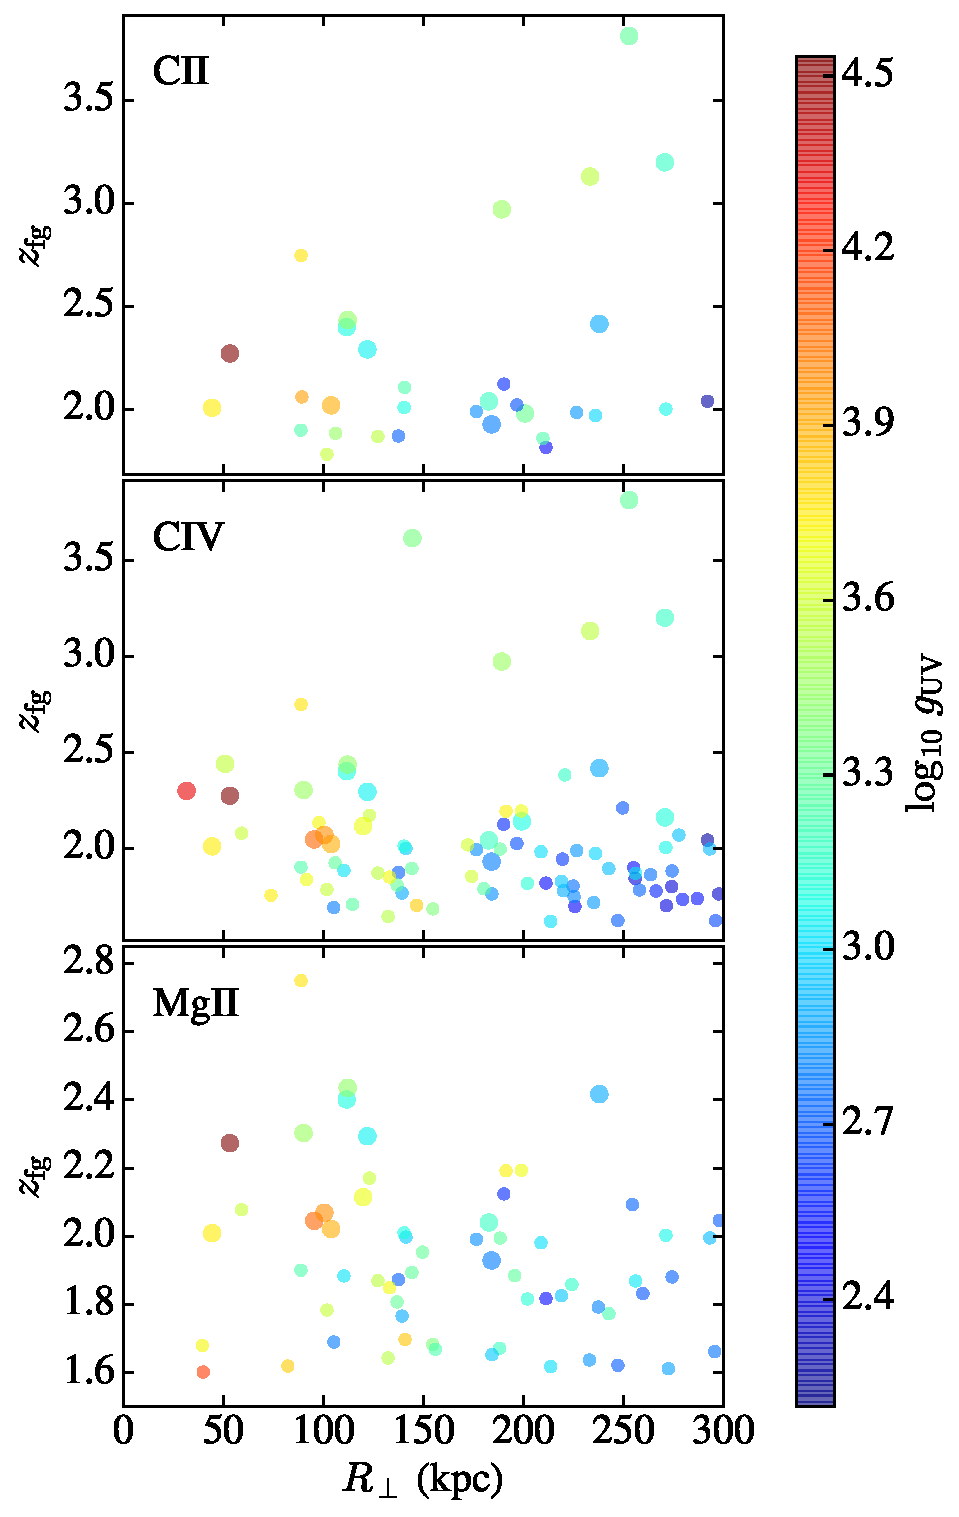
\includegraphics[width=3.5in]{Figures/fig_experiment.pdf}
%\includegraphics[width=5in,angle=90]{../Figuref1.eps}
\caption{These panels summarize properties of the QPQ9 dataset. The QPQ survey selects 
quasar pairs of projected separation $R_\perp < 300$\,kpc and $z_{\rm fg}>1.6$. Assuming that the 
foreground quasars emit isotropically and at a distance equal to the impact parameter, we estimate 
enhancement in the UV flux relative to the extragalactic UV background $g_{\rm UV}$. Smaller 
symbols correspond to foreground quasars with the most precise redshift measurement from 
[\ion{O}{3}]\,5007 emission, while larger symbols correspond to foreground quasars with redshift 
measurement from \ion{Mg}{2}\,2796, H$\alpha$, or H$\beta$ emission. The top panel shows 
quasar pairs with coverage of \ion{C}{2}\,1334 at $z_{\rm fg}$ in the background quasar spectra. 
The middle panel shows pairs with coverage of \ion{C}{4}\,1548. The bottom panel shows 
pairs with coverage of \ion{Mg}{2}\,2796. 
}
\label{fig:experiment}
\end{figure}

\begin{figure}
%\includegraphics[width=5in]{Figures/fig_simple_stack.pdf}
%\includegraphics[width=5in,angle=90]{f2.eps}
\caption{Simple stack
}
\label{fig:stack}
\end{figure}

\end{document}
